%----------------------------------------------------------------------------------------
%	PACKAGES AND OTHER DOCUMENT CONFIGURATIONS
%----------------------------------------------------------------------------------------

\documentclass[a4paper,11pt]{article} % Font and paper size

%----------------------------------------------------------------------------------------
%	PACKAGES AND OTHER DOCUMENT CONFIGURATIONS
%----------------------------------------------------------------------------------------

\usepackage[utf8]{inputenc} % Required for inputting international characters
\usepackage[T1]{fontenc} % Output font encoding for international characters
\usepackage[italian]{babel} % Italian dictionary


\usepackage[table]{xcolor} % Required for custom colors
\usepackage{gensymb}
\usepackage{amsmath}
\usepackage{bm}
\usepackage{tikz}
\usepackage{hhline}
\usepackage{listings}
\usepackage{enumitem}

%\usepackage[margin=2cm, includefoot]{geometry} % Modify margins
\usepackage{fancyhdr}
\usepackage{rotating}
\usepackage[hidelinks]{hyperref} % Hyperlinks

\usepackage[none]{hyphenat}% Non spezza le parole nelle tabelle
\usepackage{array}

\usepackage{graphicx} % Required for figures
\usepackage{float}
\usepackage{wrapfig}
\usepackage{caption}
\usepackage{subcaption}

%pagestyle
\pagestyle{fancy}
\fancyhead{}
\fancyfoot{}
\fancyfoot[R]{\thepage}
\renewcommand{\headrulewidth}{0pt}



\usepackage{xfrac}
\usepackage{amssymb}

\usepackage{multicol}
\usepackage{multirow}

\usepackage[toc, page]{appendix}
\usepackage{booktabs}
\usepackage{siunitx}


%----------------------------------------------------------------------------------------
%	NEW COMMANDS
%----------------------------------------------------------------------------------------

\newcommand{\restr}[2]{{% we make the whole thing an ordinary symbol
\left.\kern-\nulldelimiterspace % automatically resize the bar with \right
#1 % the function

\right|_{#2} % this is the delimiter
}}

\newcommand{\tnhl}{\tabularnewline\hline}
\newcommand{\tn}{\tabularnewline}
\newcolumntype{x}[1]{%
	>{\centering\hspace{0pt}}p{#1}}%


 % Include the file specifying document layout and packages


%----------------------------------------------------------------------------------------
%	GENERAL INFORMATION 
%----------------------------------------------------------------------------------------

\newcommand{\labcourse}{Laboratorio di Fisica}
\newcommand{\teacher}{Docenti: Prof. A. Garfagnini - Prof. M. Lunardon}
\newcommand{\laurea}{Corso di Laurea in Fisica}
\newcommand{\channel}{Canale 1 A-L}
\newcommand{\academicyear}{Anno Accademico 2020/2021}
\newcommand{\labexp}{Esperienza di Laboratorio}
\newcommand{\exptitle}{Amplificatori Operazionali \& Calibrazione Arduino}
\newcommand{\expobj}{Obiettivo dell'Esperienza}
\newcommand{\objectives}{Verificare la linearità di un amplificatore operazionale.}
\newcommand{\objectivess}{Misurare l'amplificazione di un circuito con amplificatore operazionale.}
\newcommand{\objectivesss}{Misurare la frequenza di taglio di un circuito derivatore con amplificatore operazionale.}
\newcommand{\objectivessss}{Calibrare una scheda Arduino Due}
\newcommand{\turno}{Turno T2}
\newcommand{\name}{Nicolò Lai}
\newcommand{\matricola}{1193976}
\newcommand{\mail}{nicolo.lai@studenti.unipd.it}
\newcommand{\consegna}{Data di consegna}
\newcommand{\data}{?/11/2020}


%----------------------------------------------------------------------------------------
%	DOCUMENT 
%----------------------------------------------------------------------------------------

\begin{document}
\def\sectionautorefname{Sezione} 
\def\subsectionautorefname{Sezione} 
\def\subsubsectionautorefname{Sezione}

%----------------------------------------------------------------------------------------
%	TITLE PAGE
%----------------------------------------------------------------------------------------

	\begin{titlepage}

		\begin{center}
			\Huge{\bfseries \labcourse}\\
				
			\LARGE \teacher \\
			\Large \laurea\\
			\Large \channel\\
			\Large \academicyear\\
			[1cm] 
			\line(1,0){400}\\
			[2cm]
				
			\textsc{\huge{\bfseries \labexp}}\\
			\huge{\exptitle}\\
			[2mm] \line(1,0){300}\\
			[3mm]

			\textsc{\Large{\bfseries \expobj}}\\
			\large{
				\objectives\\
				\objectivess\\
				\objectivesss\\
				\objectivessss
			}\\
			[7.5cm]
		\end{center}
		
		
		\begin{flushleft}
			\textsc{\Large \turno}\\
			[0.5cm] \textsc{\large {\bfseries \name}} \\ 
			\indent\large \matricola \\ 
			\indent\large \mail \\
		\end{flushleft}
			
						
		\begin{flushright}
				\textsc{\Large\consegna}\\
				\textsc{\large \data}					
		\end{flushright}
				
	\end{titlepage}
\cleardoublepage


%----------------------------------------------------------------------------------------
%	APPARATO SPERIMENTALE
%----------------------------------------------------------------------------------------

\section{Strumentazione e Componenti}\label{s:strumenti}

\begin{itemize}
	\item \textbf{Oscilloscopio} (Tektronix TBS1102B): Lo strumento presenta un'accuratezza sul guadagno verticale $\Delta_{g}$ pari
	al 3\% del valore letto (errore massimo) ed è \textit{generalmente} il contributo più significativo. L'incertezza di
	guadagno sui tempi si assume trascurabile. L'accuratezza che tiene conto degli effetti di risoluzione e imprecisione
	della traccia $\Delta_{l}$ è di 1/10 di divisione su tutta la scala di lettura (errore massimo), uguale sia per le tensioni sia
	per i tempi.

	\item \textbf{Generatore di funzioni} (Tektronix AFG1022)

	\item  \textbf{Alimentatore di tensione continua}: Lo strumento presenta due uscite con erogazione di tensione tra 0
	e 20 \si{\volt} e un'uscita con erogazione fissata a 5 \si{\volt}
	
	\item \textbf{Multimetro digitale} (Metrix MTX3292): Si riporta l'accuratezza dello strumento, per misure di
	resistenza e di capacità, relativa unicamente ai fondoscala utilizzati nell'esperienza.

	\begin{table}[H]
		\small
		\centering
		\begin{tabular}{x{2cm} x{3cm} x{3cm} } \toprule[0.5px]\toprule[0.1px]
			
			\multicolumn{3}{c}{Accuratezza Metrix MTX3292}\tn
			\midrule[0.1px]
			
			F.S. & Precisione & Risoluzione \tn
			
			\addlinespace
			
			1   \si{k\ohm} & 0.10\% + 8  & 0.01 \si{\ohm}  \tn 10  \si{k\ohm} & 0.07\% + 8  & 0.1  \si{\ohm}  \tn 100
			\si{k\ohm} & 0.07\% + 8  & 1 \si{\ohm}  \tn

			
			\addlinespace

			1000 \si{p\farad}         & 2.5\% + 15  & 1 \si{p\farad}   \tn
			
			\bottomrule[0.5px]
			
			
		\end{tabular}
		\caption{Per i fondoscala indicati si riportano la precisione (contributo di scala in percentuale e contributo
		di lettura sul digit meno significativo) e la risoluzione dello strumento.}
		\label{t:metrix}
	\end{table}	 

	\item \textbf{Componenti circuitali} (Resistori e Condensatori): Si riportano i valori delle resistenze e capacità
	utilizzate per l'assemblamento dei circuiti utilizzati nel corso dell'esperienza, misurate preliminarmente con il
	multimetro digitale Metrix. 

	\begin{table}[H]
		\small
		\centering
		\begin{tabular}{x{2cm} x{3cm} x{3cm} } \toprule[0.5px]\toprule[0.1px]
			
			\multicolumn{3}{c}{Resistori e Condensatori}\tn
			\midrule[0.1px]
			
			Resistenza & Valore & F.S. \tn
			
			\addlinespace
			
			$R_f$ & $(82.46 \pm 0.03)\,\si{k\ohm}$ & $100\,\si{k\ohm}$ \tn

			$R_1$ & $(8.089 \pm 0.003)\,\si{k\ohm}$ & $10\,\si{k\ohm}$ \tn

			$R_3$ & $(46.54 \pm 0.05)\,\si{\ohm}$ & $1\,\si{k\ohm}$ \tn
		
			\addlinespace

			\midrule[0.1px]
			
			Capacità & Valore & F.S. \tn
			
			\addlinespace

			$C_1$  & $(977 \pm 17)\,\si{p\farad}$  & $1000\,\si{p\farad}$   \tn
			
			\bottomrule[0.5px]
			
		\end{tabular}
		\caption{In tabella si indicano le componenti circuitali (resistori e capacità) utilizzando delle label
		specifiche per ciascuna di esse: questa notazione è costante nel corso dell'esperienza.}
		\label{t:direct_measures}
	\end{table}	

	\item \textbf{Circuito integrato TL082C} (Due Amplificatori Operazionali): essendo gli amplificatori operazionali
	delle componenti circuitali attive, esse devono essere alimentate. Si utilizza dunque il generatore di tensione
	continua con $V_{\text{cc}} = +15\,\si{\volt}$ e $V_{\text{ee}}=-15\,\si{\volt}$ per l'alimentazione
	dell'amplificatore operazionale utilizzato nell'esperienza. Nel corso di quest'ultima, si assume un comportamento
	\textit{ideale} dell'amplificatore operazionale, ovvero che il polo positivo ed il polo negativo si trovino
	allo stesso potenziale.
	
	\item \textbf{Scheda Arduino Due}
\end{itemize}

\cleardoublepage


%----------------------------------------------------------------------------------------
%	AMPLIFICATORE OPERAZIONALE INVERTENTE
%----------------------------------------------------------------------------------------

\section{Amplificatore Operazionale Invertente}
In questa sezione ci si propone di studiare il comportamento di un circuito puramente resistivo comprendente un
amplificatore operazionale in configurazione invertente (polo positivo a massa, polo negativo collegato al segnale in
ingresso). Si vuole in particolare verificare la sua linearità e stimare l'amplificazione del circuito come grandezza
derivata sia partendo dalle misure dirette delle resistenze sia come parametro di un'interpolazione lineare di misure
acquisite con l'oscilloscopio. 


%----------------------------------------------------------------------------------------
%	CONFIGURAZIONE SPERIMENTALE
%----------------------------------------------------------------------------------------

\subsection{Configurazione Sperimentale}

Si inizia assemblando il circuito rappresentato in  \autoref{i:opamp_circuit}, utilizzando le resistenze $R_f$, $R_1$,
$R_3$ e l'amplificatore operazionale. La resistenza $R_g$ rappresenta la resistenza interna del generatore, non nulla in
quanto ci si trova in condizioni di non idealità. 

\begin{figure}[H]
	\centering
	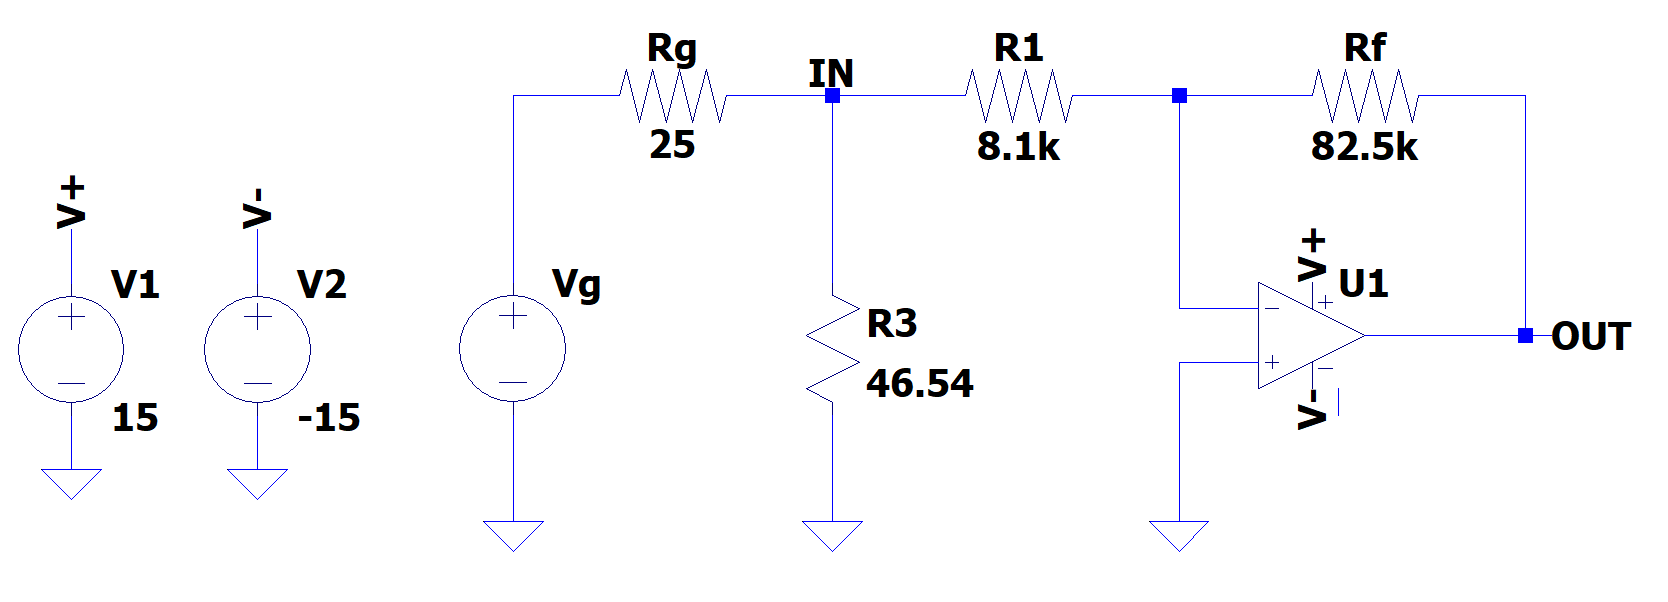
\includegraphics[width=15cm]{../Simulations/OpAmp/circuit_image_nosim.png}
	\caption{Rappresentazione a variabili concentrate del circuito assemblato in laboratorio.}
	\label{i:opamp_circuit}
\end{figure}

\noindent Il segnale viene prelevato nei punti \textit{IN} e \textit{OUT} evidenziati nello schema in
\autoref{i:opamp_circuit} (e verrà in seguito richiamato rispettivamente come $V_{\text{in}}$ e $V_{\text{out}}$)
utilizzando due sonde con fattore di attenuazione 10X. Nel canale CH1 dell'oscilloscopio viene visualizzato il segnale
in ingresso $V_{\text{in}}$, mentre il segnale in uscita $V_{\text{out}}$ è prelevato dalla sonda collegata al canale
CH2. Per entrambi i canali viene configurata l'attenuazione sonda 10X nelle impostazioni dell'oscilloscopio, in modo da
compensare la riduzione del segnale dovuta alle sonde e visualizzare quindi nel display il segnale reale. Il generatore
di funzioni viene poi configurato in modalità "50 Ohm", in modo che l'impedenza d'uscita del generatore sia comparabile
con $R_3\approx 50\,\si{\ohm}$. Ci si aspetta così di trovare una tensione in ingresso $V_{\text{in}}$ in accordo con la
tensione nominale erogata dal generatore. Si imposta infine il generatore di funzioni in modo da erogare un segnale di
tipo sinusoidale con frequenza $f_{\text{gen}}=1\,\si{k\hertz}$ e di ampiezza variabile.

%----------------------------------------------------------------------------------------
%	AMPLIFICAZIONE ATTESA
%----------------------------------------------------------------------------------------

\subsection{Amplificazione Attesa}\label{s:guadagno}
Facendo riferimento ai valori delle resistenze  $R_f$ ed $R_1$ riportate in  \autoref{t:direct_measures}, si vuole
calcolare il guadagno $G$ atteso

\begin{align}\label{e:guadagno}
	G&=\left|-\frac{R_{\text{f}}}{R_{1}}\right| 
	&
	\sigma_{G}&=\sqrt{	\left(	\frac{	1	}{	R_{1}	}	\right)^2	\sigma_{R_{\text{f}}}^2	
	+	\left(	\frac{	R_{\text{f}}	}{	R_{1}^2	}	\right)\sigma_{R_{1}}^2	}	
\end{align}

\noindent dove il segno meno è dovuto all'operazionale posto in configurazione invertente: questo comporta allora un
segnale  $V_{\text{out}}$ "invertito" (cioè ci si aspetta che i massimi del segnale in ingresso corrispondano a minimi
del segnale in uscita e viceversa) e amplificato di un fattore 

\begin{equation}
	G = 10.194 \pm 0.006.
\end{equation}

%----------------------------------------------------------------------------------------
%	ACQUISIZIONE MISURE
%----------------------------------------------------------------------------------------

\subsection{Acquisizione Misure}
Al fine di verificare la linearità dell'amplificatore operazionale e stimare l'amplificazione del circuito, si decide di
far variare la tensione in ingresso impostando valori crescenti di ampiezza del segnale erogato dal generatore di
funzioni. Per ciascuno di questi valori di tensione si acquisisce la misura di un massimo e di un minimo sia del segnale
$V_{\text{in}}$ sia del segnale $V_{\text{out}}$ sfruttando i cursori orizzontali dell'oscilloscopio. In questo modo, si
ottiene un campione di coppie ($V_{\text{in}}$, $V_{\text{out}}$) che ci si aspetta segua un andamento lineare (assumendo
la linearità dell'amplificatore operazionale). I valori di tensione $V_{\text{gen}}$, $V_{\text{in}}$, $V_{\text{out}}$ e
le relative scale di misura sono riportate in  \autoref{t:osc_measures}. Si associa inoltre un'incertezza alle misure
di $V_{\text{in}}$ e $V_{\text{out}}$ data da  \autoref{e:osc}.\\

%----------------------------------------------------------------------------------------
%	SIMULAZIONE SPICE PRELIMINARE
%----------------------------------------------------------------------------------------

\subsection{Simulazione Spice Preliminare}\label{s:spice} Prima di procedere con l'analisi dati, si decide di simulare
la risposta del circuito utilizzando il programma LTSpice. Si sceglie di effettuare la simulazione considerando due
ampiezze in ingresso significative: per la prima si imposta dal generatore un'ampiezza $V_{\text{gen}}=1\,\si{\volt}$
mentre per la seconda $V_{\text{gen}}=4\,\si{\volt}$. Questa scelta è dettata dal fatto che l'amplificatore
operazionale, essendo una componente attiva del circuito, non può dare in output una tensione maggiore di quanta ne
riceve in alimentazione per conservazione dell'energia: ci si aspetta allora di trovare una situazione di saturazione
del segnale in uscita e che questa inizi a manifestarsi attorno ad un valore nominale di tensione
$V\text{pp}_{\text{gen}}=3\,\si{\volt}$ in quanto, avendo un guadagno di circa 10, il segnale in uscita non può superare
i $30\,\si{\volt}$ picco picco.

\begin{figure}[H]
	\centering
	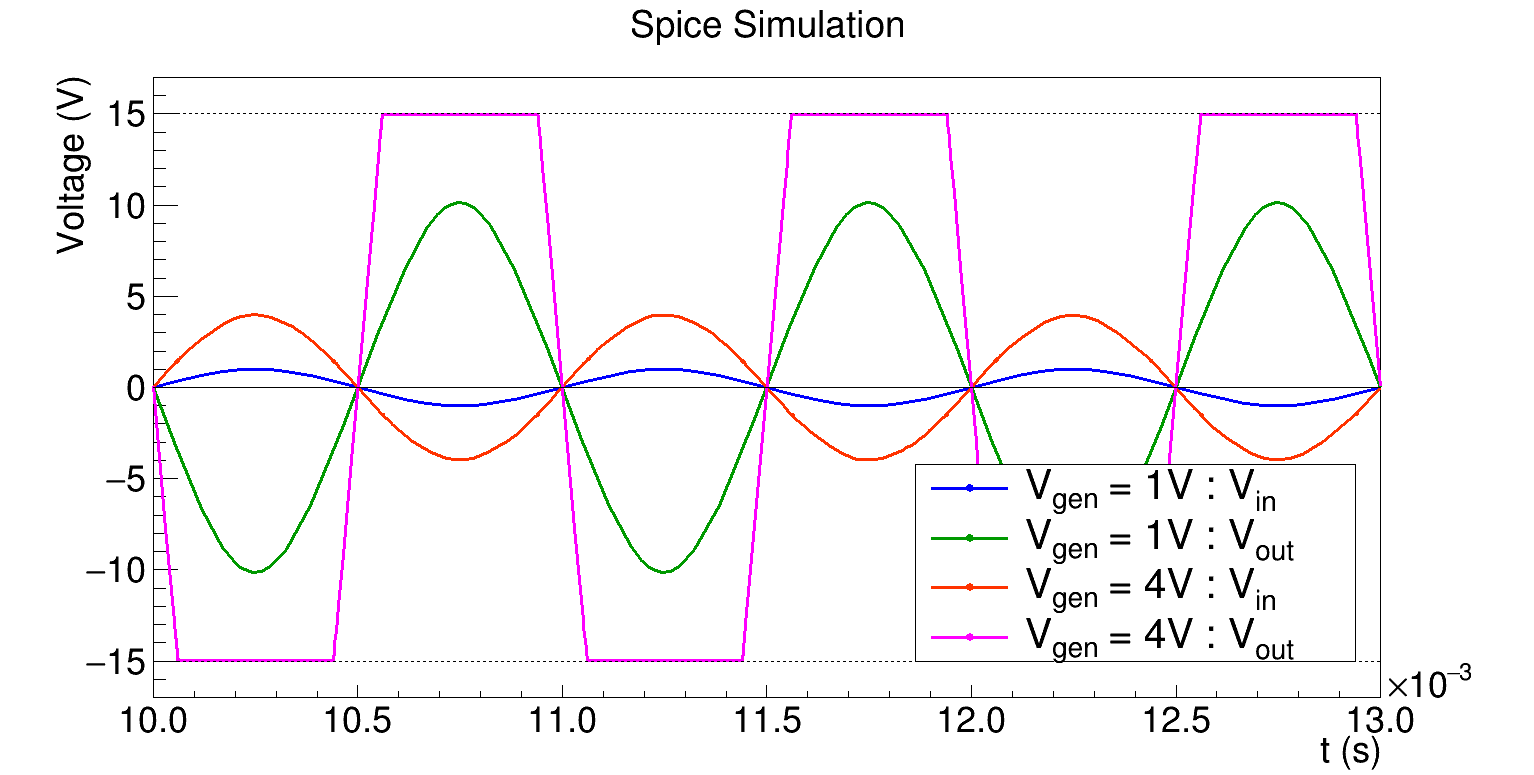
\includegraphics[width=15cm]{../Plots/Report_Plots/opamp_spice_1V_4V.png}
	\caption{Simulazione Spice della risposta del circuito ad una tensione sinusoidale in ingresso di frequenza
	$f_{\text{gen}}=1\,\si{k\hertz}$ e ampiezza $V_{\text{gen}}=1\,\si{\volt}$ oppure $V_{\text{gen}}=4\,\si{\volt}$}
	\label{i:opamp_simulation}
\end{figure}

\noindent Dal grafico si evince chiaramente come erogando $V_{\text{gen}}=1\,\si{\volt}$ il segnale viene amplificato
correttamente di circa un fattore 10 mantenendo la forma sinusoidale, mentre erogando $V_{\text{gen}}=4\,\si{\volt}$ il
segnale in uscita presenta i picchi tagliati esattamente a livello $V_{\text{sat}}=\pm 15\,\si{\volt}$, ovvero le
tensioni di alimentazione fornite all'operazionale. Inoltre, come anticipato in \autoref{s:guadagno}, si può osservare
il comportamento invertente dell'amplificatore operazionale: ad un massimo di $V_{\text{in}}$ corrisponde un minimo di
$V_{\text{out}}$ e viceversa.\\


%----------------------------------------------------------------------------------------
%	DATI E ANALISI
%----------------------------------------------------------------------------------------

\subsection{Dati e Analisi}
In questa sezione si vuole inizialmente rappresentare le misure acquisite in laboratorio, sia riportandole in tabella
sia utilizzando un grafico esplorativo di $V_{\text{out}}$ contro $V_{\text{in}}$, per cercare di estrarre informazioni
di carattere generale sui dati a disposizione. Successivamente, si vuole invece caratterizzare la linearità
dell'amplificatore operazionale ed il guadagno del circuito in termini statistici, focalizzandosi sullo studio di interpolazioni
lineari. Rappresentando in un grafico $V_{\text{out}}$ contro $V_{\text{in}}$, infatti, è possibile ricavare
l'amplificazione come il coefficiente angolare di una retta che interpola i dati: dalla bontà del fit si riesce inoltre a
studiare le proprietà di linearità del sistema in questione.

%----------------------------------------------------------------------------------------
%	DATISET
%----------------------------------------------------------------------------------------

\subsubsection{Dataset}
Si riportano in  \autoref{t:osc_measures} le misure acquisite con l'oscilloscopio, alle quali è stata associata un'incertezza

\begin{equation}\label{e:osc}
	\sigma_{V} = \sqrt{ (\sigma_{l}\times\text{V/div})^2 + (\sigma_{g}\times\text{measure})^2 }
\end{equation}

\noindent dove $\sigma_{l}=\Delta_{l}/\sqrt{6}$ e $\sigma_{g}=\Delta_{g}/\sqrt{6}$ (assumendo una distribuzione
triangolare) rappresentano l'incertezza di lettura e di guadagno associati all'oscilloscopio (si rimanda a 
\autoref{s:strumenti} per i valori di $\Delta_{l}$ e $\Delta_{g}$), V/div rappresenta la scala di acquisizione della misura,
ovvero quanti Volt sono rappresentati in una divisione dello schermo dell'oscilloscopio, mentre "measure" rappresenta la
misura stessa.

\begin{table}[H]
	\centering
	\footnotesize
	\begin{tabular}{x{2cm} x{3cm} x{3.2cm} x{3cm} x{3.2cm}} 

		\toprule[0.5px]
		\toprule[0.1px]
		
		\multicolumn{5}{c}{Misure Acquisite con l'Oscilloscopio}\tn
		\midrule[0.1px]

		\multicolumn{5}{c}{Misure dei Massimi}\tn

		\addlinespace
		
		$V\text{{pp}}_{\text{gen}}$ (V)& $V_{\text{in}}$ (V)& Scala $V_{\text{in}}$ (V/div)& $V_{\text{out}}$ (V)& Scala
		$V_{\text{out}}$ (V/div)\tn
		
		\addlinespace
		
		$	0.20		$&$	0.106 \pm	0.003	$&$	0.050	$&$	1.00 \pm	0.02	$&$	0.324	$\tn
		$	0.50		$&$	0.252 \pm	0.006	$&$	0.100	$&$	2.48 \pm	0.05	$&$	1.00	$\tn
		$	0.80		$&$	0.400 \pm	0.010	$&$	0.200	$&$	4.00 \pm	0.10	$&$	2.00	$\tn
		$	1.00		$&$	0.496 \pm	0.011	$&$	0.200	$&$	4.96 \pm	0.11	$&$	2.00	$\tn
		$	1.50		$&$	0.744 \pm	0.014	$&$	0.200	$&$	7.44 \pm	0.14	$&$	2.00	$\tn
		$	1.80		$&$	0.907 \pm	0.019	$&$	0.324	$&$	8.98 \pm	0.19	$&$	3.40	$\tn
		$	2.00		$&$	1.01 \pm	0.02	$&$	0.324	$&$	9.9  \pm	0.2		$&$	3.40	$\tn
		$	2.30		$&$	1.16 \pm	0.02	$&$	0.376	$&$	11.4 \pm	0.2		$&$	3.80	$\tn
		$	2.60		$&$	1.29 \pm	0.03	$&$	0.436	$&$	13.0 \pm	0.3		$&$	4.52	$\tn
		$	3.00		$&$	1.50 \pm	0.03	$&$	0.480	$&$	14.4 \pm	0.3		$&$	4.52	$\tn
		$	3.20		$&$	1.61 \pm	0.03	$&$	0.630	$&$	14.7 \pm	0.3		$&$	5.60	$\tn	
		$	3.50		$&$	1.77 \pm	0.04	$&$	0.660	$&$	14.7 \pm	0.3		$&$	5.60	$\tn
		
	
		\addlinespace

		\midrule[0.1px]
		
		\multicolumn{5}{c}{Misure dei Minimi}\tn

		\addlinespace
		
		$V\text{{pp}}_{\text{gen}}$ (V)& $V_{\text{in}}$ (V)& Scala $V_{\text{in}}$ (V/div)& $V_{\text{out}}$ (V)& Scala
		$V_{\text{out}}$ (V/div)\tn

		\addlinespace

		$	0.20		$&$	-0.102 \pm	0.003	$&$	0.050	$&$	-0.97 \pm	0.02	$&$	0.324	$\tn
		$	0.50		$&$	-0.252 \pm	0.006	$&$	0.100	$&$	-2.48 \pm	0.05	$&$	1.00	$\tn
		$	0.80		$&$	-0.400 \pm	0.010	$&$	0.200	$&$	-3.92 \pm	0.10	$&$	2.00	$\tn
		$	1.00		$&$	-0.496 \pm	0.011	$&$	0.200	$&$	-4.96 \pm	0.11	$&$	2.00	$\tn
		$	1.50		$&$	-0.736 \pm	0.014	$&$	0.200	$&$	-7.36 \pm	0.14	$&$	2.00	$\tn
		$	1.80		$&$	-0.881 \pm	0.019	$&$	0.324	$&$	-8.98 \pm	0.19	$&$	3.40	$\tn
		$	2.00		$&$	-0.98  \pm	0.02	$&$	0.324	$&$	-10.0 \pm	0.2		$&$	3.40	$\tn
		$	2.30		$&$	-1.13  \pm	0.02	$&$	0.376	$&$	-11.5 \pm	0.2		$&$	3.80	$\tn
		$	2.60		$&$	-1.29  \pm	0.03	$&$	0.436	$&$	-13.0 \pm	0.3		$&$	4.52	$\tn
		$	3.00		$&$	-1.48  \pm	0.03	$&$	0.480	$&$	-14.1 \pm	0.3		$&$	4.52	$\tn
		$	3.20		$&$	-1.59  \pm	0.03	$&$	0.630	$&$	-14.8 \pm	0.3		$&$	5.60	$\tn	
		$	3.50		$&$	-1.72  \pm	0.04	$&$	0.660	$&$	-14.8 \pm	0.3		$&$	5.60	$\tn
		
		
		\bottomrule[0.5px]
		
	\end{tabular}
	\caption{Vengono rappresentate in tabella le misure sperimentali acquisite con i cursori dell'oscilloscopio 
				con l'incertezza ad esse associata e la scala di acquisizione della misura.}
	\label{t:osc_measures}
\end{table}	

\noindent  Osservando la colonna relativa alla tensione in ingresso $V_{\text{in}}$, si nota come sia conforme alla
tensione nominale erogata dal generatore di funzioni: questo è sicuramente indice di una corretta acquisizione del
segnale in ingresso e di una corretta configurazione del generatore (\textit{modalità "50 Ohm"}) e dell'oscilloscopio
(\textit{attenuazione sonda 10X}). Osservando invece la colonna relativa a $V_{\text{out}}$ si nota un'amplificazione
conforme alle aspettative (circa un fattore 10). Inoltre, si osserva come le ultime misure per entrambi i campioni, cioè
quelle con tensione nominale $V\text{pp}_{\text{gen}}$ maggiore, tendano a stabilizzarsi attorno a circa
$V_{\text{sat}}=\pm15\,\si{\volt}$, ovvero la tensione massima che l'amplificatore operazionale può fornire in output.
Come da aspettative, riportate in \autoref{s:spice}, questo fenomeno di stabilizzazione attorno a $V_{\text{sat}}$
inizia a manifestarsi attorno ad una tensione erogata dal generatore di circa $V\text{pp}_{\text{gen}}=3\,\si{\volt}$.\\
Per meglio chiarificare l'andamento delle misure ed il fenomeno di saturazione, si riportano nel grafico in
\autoref{i:opamp_eda} le coppie ($V_{\text{in}}$, $V_{\text{out}}$): queste vengono quindi interpolate con una retta del
tipo $y=a+bx$ al fine di osservare l'andamento dei residui. Per quanto riguarda gli errori associati alle misure, si
rappresentano quelli calcolati usando \autoref{e:osc} e mostrati in \autoref{t:osc_measures}, al fine di osservare
(\textit{approssimativamente}) l'ellisse di incertezza dei dati.

\begin{figure}[H]
	\centering
	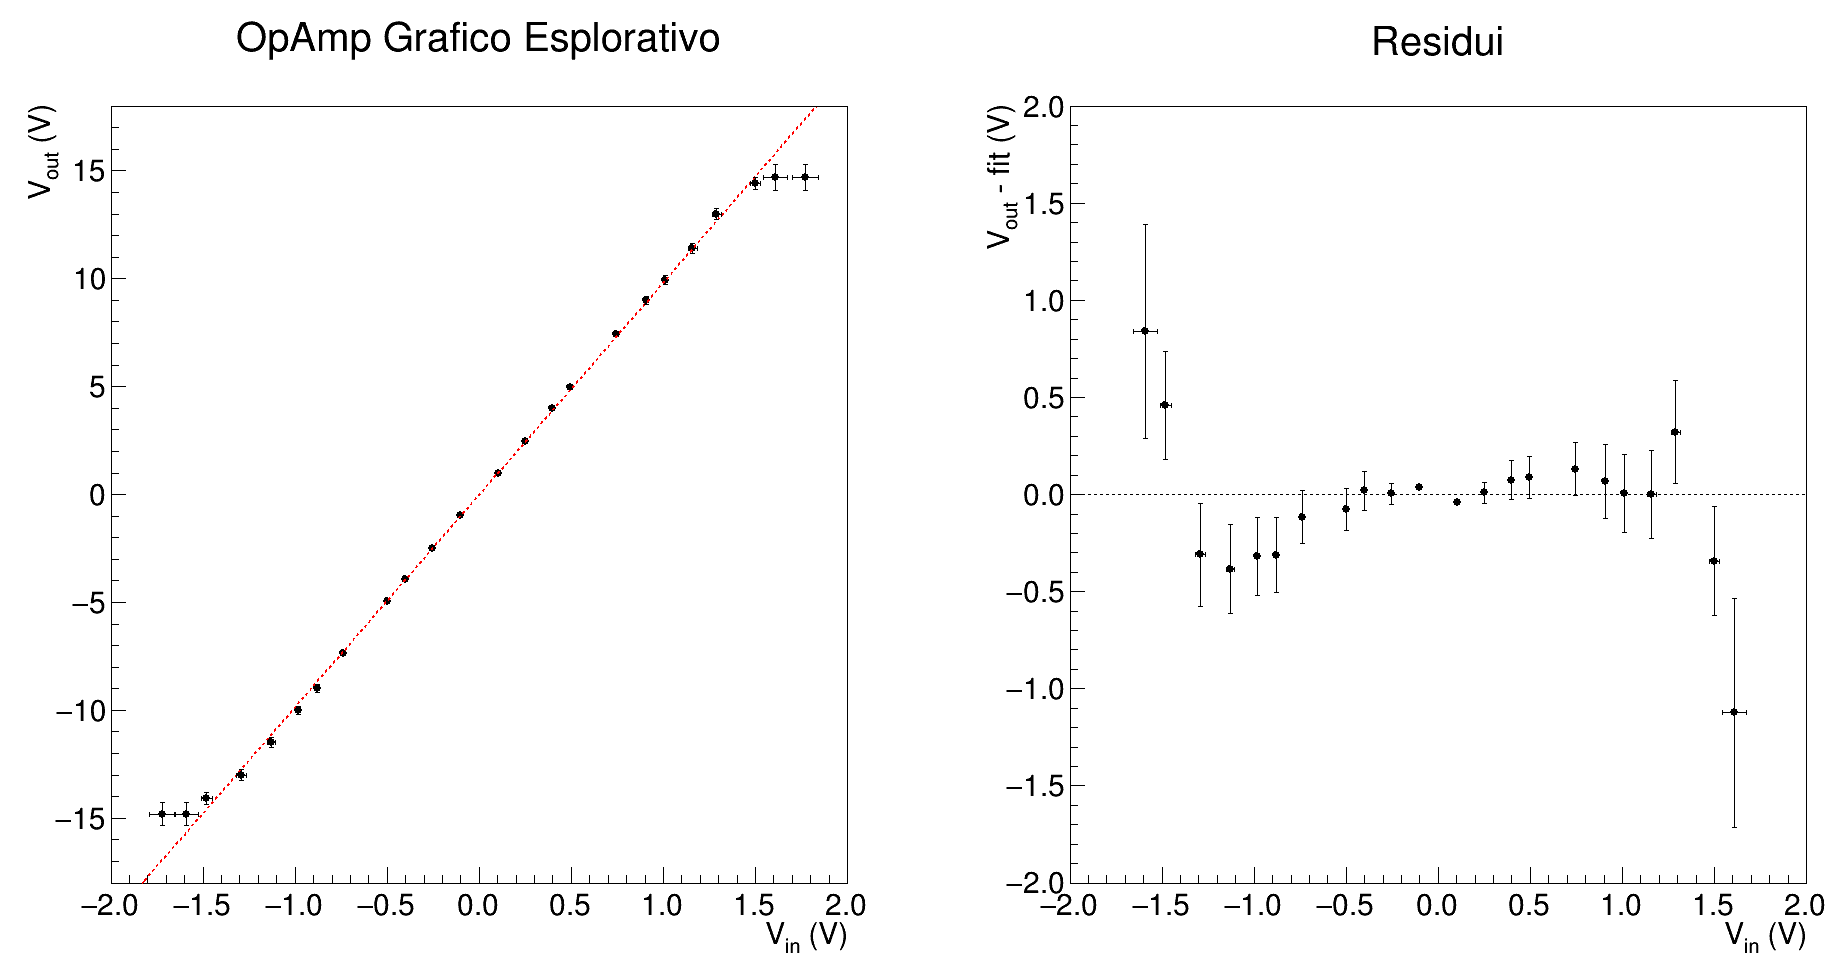
\includegraphics[width=15cm]{../Plots/Report_Plots/opamp_plot_alldata_eda.png}
	\caption{A sinistra: grafico delle coppie ($V_{\text{in}}$, $V_{\text{out}}$) interpolate linearmente da una retta
	del tipo $y=a+bx$. A destra: grafico dei residui.}
	\label{i:opamp_eda}
\end{figure}

\noindent Dal grafico a sinistra si nota immediatamente il fenomeno di saturazione del segnale in uscita a
$V_{\text{sat}}=\pm15\,\si{\volt}$: i tre punti finali di massimo e minimo tendono a stabilizzarsi piuttosto che seguire
il trend lineare, fedelmente rispettato dai restanti punti del grafico. Dal grafico dei residui si può osservare lo
stesso fenomeno: la zona centrale risulta essere distribuita ragionevolmente attorno allo zero, mentre le code tendono a
distanziarsi anche notevolmente. Da questo si deduce dunque che i tre punti finali di massimo e di minimo sono da
considerarsi degli outliers rispetto al trend lineare delle misure rimanenti: al fine di caratterizzare la
linearità dell'amplificatore operazionale e di calcolare l'amplificazione del circuito, dunque, gli outliers non
verranno considerati.

%----------------------------------------------------------------------------------------
%	PRELIMIARY FIT
%----------------------------------------------------------------------------------------

\subsubsection{Interpolazioni Preliminari}\label{s:pre} Si procede ora considerando il campione di misure dei massimi ed
il campione di misure dei minimi separatamente, in quanto a priori non si ha la certezza che queste risentano della
stessa amplificazione e che non sia presente una sistematica di offset/shift verticale tra i due dataset. Si cercherà in
seguito di caratterizzare l'accordo tra i due dataset studiando la compatibilità tra i coefficienti angolari e tra le
intercette della retta interpolante. Osservando le misure in  \autoref{t:osc_measures} si nota come le incertezze su
$V_{\text{in}}$ siano generalmente un ordine di grandezza inferiori rispetto a quelle su $V_{\text{out}}$: le prime non
sono quindi trascurabili rispetto alle seconde. Per tenere conto dell'incertezza su $V_{\text{in}}$, ci si propone
allora di effettuare un fit preliminare, nel quale si considerano unicamente gli errori su $V_{\text{out}}$, per stimare
un coefficiente angolare $m$. Questo viene poi utilizzato per proiettare gli errori di $V_{\text{in}}$ lungo l'asse
delle ordinate secondo 

\begin{equation}\label{e:proj}
	\sigma_{y} = \sqrt{	\sigma_{V_{\text{out}}}^2	+	m^2	\sigma_{V_{\text{in}}}^2	}
\end{equation}

\noindent I coefficienti angolari di interesse sono dunque riportati in  \autoref{t:pre_slopes}.

\begin{table}[H]
	\small
	\centering
	\begin{tabular}{x{4cm} x{4cm}} 

		\toprule[0.5px]
		\toprule[0.1px]
		
		\multicolumn{2}{c}{Coefficienti Angolari Preliminari}\tn
		\midrule[0.1px]

		Campione di Massimi & Campione di Minimi \tn

		\addlinespace
		
		$m=10.02\pm0.09$ & $m=10.16\pm0.09$ \tn
		
		\bottomrule[0.5px]
		
	\end{tabular}
	\caption{Valori dei coefficienti angolari restituiti dalle interpolazioni preliminari.}
	\label{t:pre_slopes}
\end{table}	

\noindent Questi due coefficienti angolari vengono adesso utilizzati per proiettare il contributo d'errore relativo a
$V_{\text{in}}$ lungo l'asse y secondo la formula in  \autoref{e:proj}.


%----------------------------------------------------------------------------------------
%	LINEARITA E AMPLIFICAZIONE
%----------------------------------------------------------------------------------------

\subsubsection{Linearità e Amplificazione}
Alla luce di quanto trovato nella sezione precedente, si ripetono le interpolazioni lineari associando ai punti un
errore dato da  \autoref{e:proj} ed i parametri restituiti dai fit sono riportati in  \autoref{t:opamp_fitres_max_min}.

\begin{table}[H]
	\centering
	\small
	\begin{tabular}{x{3cm} x{3cm} x{3cm} x{3cm}} 

		\toprule[0.5px]
		\toprule[0.1px]
		
		\multicolumn{4}{c}{Fit Parameters}\tn
		\midrule[0.1px]

		\multicolumn{4}{c}{Campione di Massimi}\tn

		\addlinespace
		
		Offset (V) & Slope & $\chi^2$/ndf & $\sigma_{\text{posteriori}}$ (V)\tn

		\addlinespace

		$-0.06\pm0.04$ & $10.02\pm0.14$ & $0.98/7$ & $0.10$ \tn

		\midrule[0.1px]
		
		\multicolumn{4}{c}{Campione di Minimi}\tn

		\addlinespace
		
		Offset (V) & Slope & $\chi^2$/ndf & $\sigma_{\text{posteriori}}$ (V) \tn

		$0.07\pm0.04$ & $10.16\pm0.14$ & $0.67/7$ & $0.07$ \tn



		\bottomrule[0.5px]
		
	\end{tabular}
	\caption{Parametri della retta interpolante, il valore del $\chi^2$ associato al fit 
	e l'errore a posteriori relativo alla distribuzione dei dati.}
	\label{t:opamp_fitres_max_min}
\end{table}	

\noindent Dai parametri presentati in  \autoref{t:opamp_fitres_max_min} si riescono ad estrarre numerose informazioni
riguardo ai due campioni di dati. Inizialmente, si vuole far notare come i due coefficienti angolari siano in ottima
compatibilità tra loro: $\lambda=0.7$. Da questo si può assumere che i due dataset risentano della stessa amplificazione
$G$, come da aspettative. Successivamente, si può notare invece che le due intercette delle rette interpolanti sono in
leggera compatibilità con lo zero ($\lambda \approx 1.5$), mentre tra loro presentano una compatibilità $\lambda=2.4$,
che fa sorgere l'idea di una possibile sistematica di shift verticale tra i due dataset. Osservando poi il valore del
$\chi^2$, si ritrova in per entrambi i campioni $\chi^2/\nu<1$ (con $\nu\equiv\text{ndf}$ il numero di gradi di libertà, che
coincide con il valore di aspettazione $E(\chi^2)$). Questo fa emergere l'ipotesi di una possibile sovrastima
dell'errore associato alle misure ed ad una conseguente sovrastima degli errori sui parametri restituiti dal fit.
Tuttavia, si ricorda che le incertezze sul guadagno verticale dell'oscilloscopio sono almeno parzialmente correlate:
questo porta dunque ad avere degli errori sulle misure che sono tra loro correlati ed un'interpolazione di tali dati
restituisce parametri con errori sottostimati (il fit non tiene conto della correlazione tra incertezze delle misure).
Si può dunque assumere che i parametri \textit{slope} e \textit{offset} riportati in \autoref{t:opamp_fitres_max_min}
siano in realtà più compatibili tra dataset di massimi e dataset di minimi rispetto a quanto riportato poco sopra,
proprio a causa di una possibile sottostima dell'errore sui parametri. Siccome allora si può assumere che i due campioni
risentano della stessa amplificazione e che non siano tra loro sfalsati verticalmente, segue un tentativo di
"unificazione" del campione di dati ed un'interpolazione lineare unica che tenga conto sia dei massimi che dei minimi.
Il grafico rappresentante i due dataset unificati con relativa interpolazione lineare è mostrato in
\autoref{i:opamp_all_proj}. 

\begin{figure}[H]
	\centering
	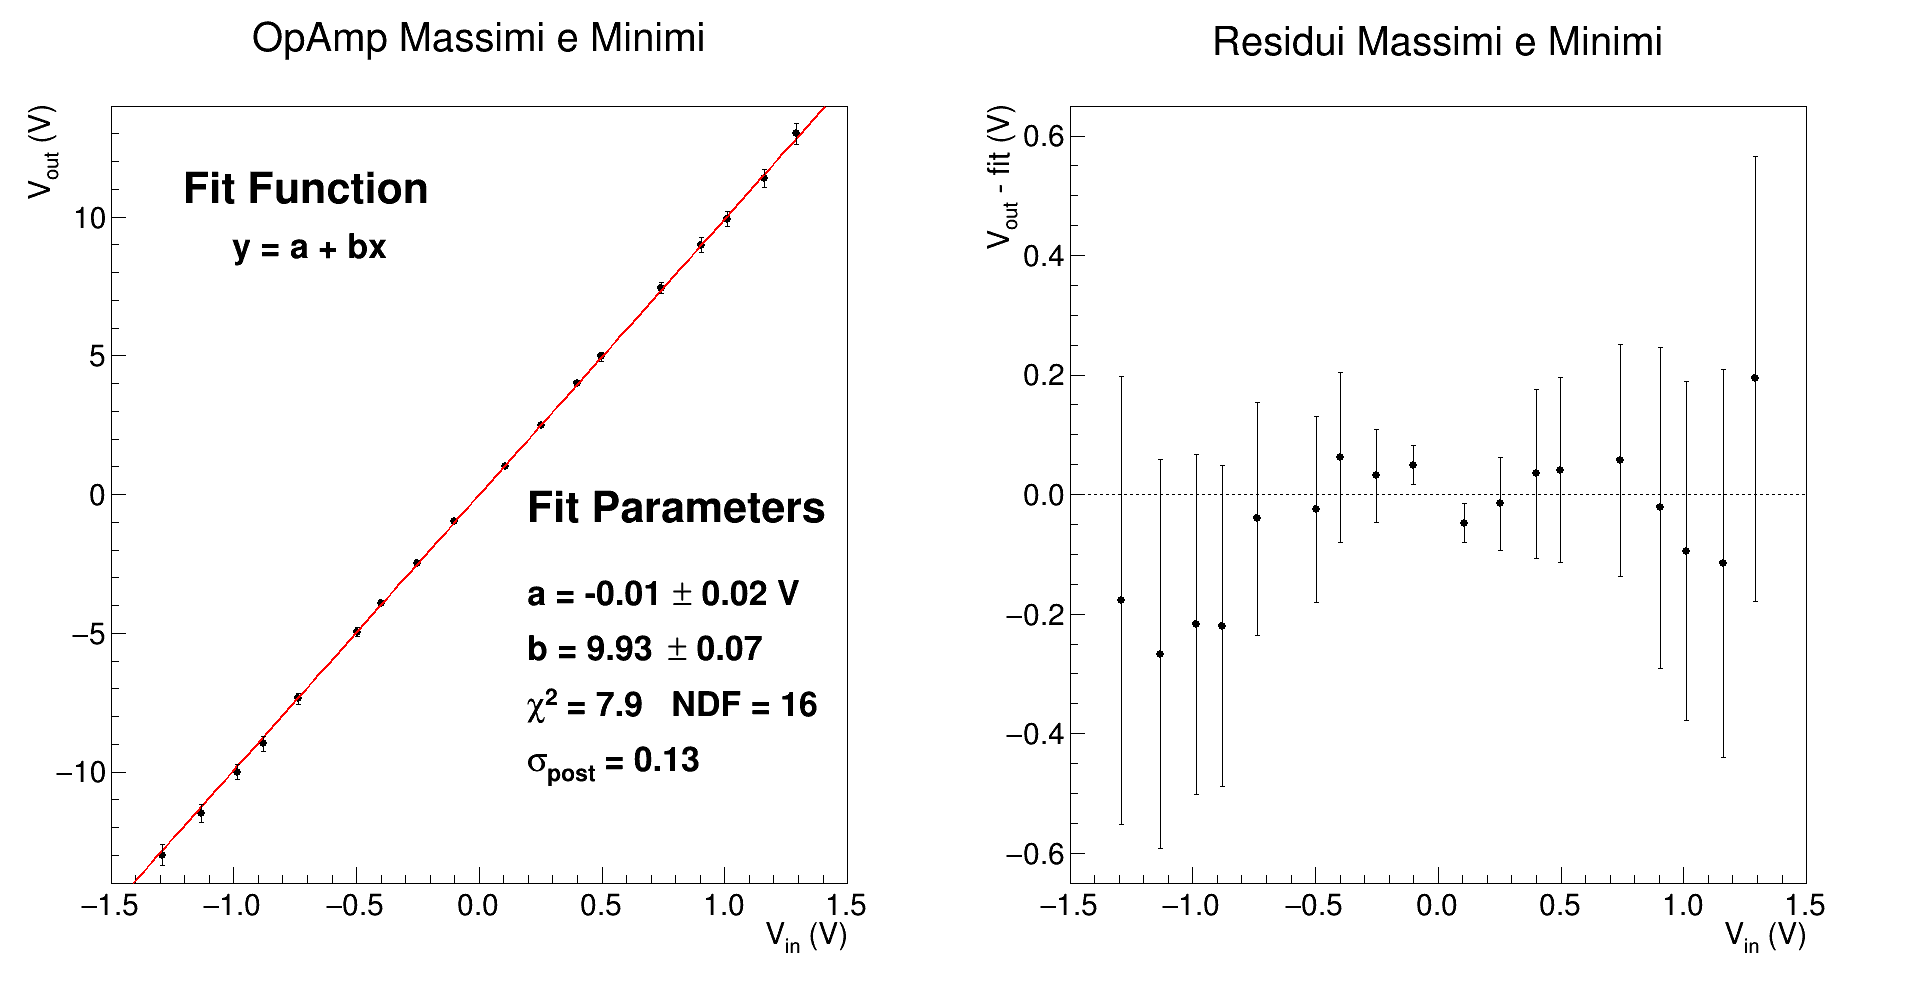
\includegraphics[width=15cm]{../Plots/Report_Plots/opamp_plot_all_projected.png}
	\caption{A sinistra: grafico rappresentante il dataset dei massimi ed il dataset dei minimi uniti assieme, 
	con relativa retta interpolante e parametri del fit. A destra: grafico dei residui $V_{\text{out}}-\text{fit}$.}
	\label{i:opamp_all_proj}
\end{figure}

\noindent I parametri restituiti dall'interpolazione sono i seguenti 

\begin{table}[H]
	\small
	\centering
	\begin{tabular}{x{3cm} x{3cm} x{3cm} x{3cm}} 

		\toprule[0.5px]
		\toprule[0.1px]
		
		\multicolumn{4}{c}{Fit Parameters}\tn
		\midrule[0.1px]

		\addlinespace
		
		Offset (V) & Slope & $\chi^2$/ndf & $\sigma_{\text{posteriori}}$ (V)\tn

		\addlinespace

		$-0.01\pm0.02$ & $9.93\pm0.07$ & $7.9/16$ & $0.13$ \tn

		\bottomrule[0.5px]
		
	\end{tabular}
	\caption{Parametri della retta interpolante, il valore del $\chi^2$ associato al fit 
	e l'errore a posteriori relativo alla distribuzione dei dati.}
	\label{t:opamp_fitres_all}
\end{table}	

\noindent Si osserva inizialmente che l'intercetta della retta interpolante è ora ben compatibile con zero, mentre il
coefficiente angolare presenta un errore relativo $\sigma_{b}/b=0.7\%$, che si può continuare ad assumere sottostimato:
la correlazione tra gli errori di scala, infatti, si può notare chiaramente dall'andamento "a farfalla" delle barre
d'errore nel grafico dei residui. Il valore del $\chi^2$ migliora leggermente rispetto alle interpolazioni dei dataset
separati: la compatibilità con il valore di aspettazione risulta essere $Z=1.4$. L'errore a posteriori, inoltre, si
trova in una zona intermedia rispetto alla gamma di errori associati alle misure: non potendo eliminare la correlazione
tra le incertezze si può affermare dunque che l'errore è in media ben stimato e l'oscilloscopio lavora entro le
specifiche. I residui, infatti, si posizionano tutti entro il loro errore, alcuni anche abbondantemente. Focalizzandosi
ora sulla stima del coefficiente angolare si nota che questo, $m=9.93\pm 0.07$, pur essendo ben compatibile con i
risultati esposti in  \autoref{t:opamp_fitres_max_min} relativi ai fit dei due campioni di misure considerati
separatamente, si trova essere sensibilmente minore di entrambi: ci si sarebbe aspettato, invece, di trovare un valore
intermedio unificando i due campioni di misure. Osservando poi il grafico dei residui, si può notare un andamento
leggermente anomalo, quasi parabolico, avente concavità rivolta verso il basso. Si ipotizza dunque che l'assunzione
fatta in precedenza riguardo la presenza di una sistematica di offset/shift verticale tra i due dataset trascurabile
necessiti di essere rivisitata. Per approfondire maggiormenta la questione, si decide di computare le grandezze "picco
picco" delle tensioni in ingresso $V_{\text{in}}$ e in uscita $V_{\text{out}}$ secondo
$V_{\text{pp}}=V^{\text{max}}-V^{\text{min}}$. Per quanto riguarda l'errore da associare alle grandezze picco picco, si
ricorda che l'oscilloscopio misura la differenza $\Delta$ tra i due cursori con una precisione ancora maggiore rispetto
alla singola misura. Si decide dunque di non aggiungere il fattore moltiplicativo $\sqrt{2}$ alla propagazione
presentata in  \autoref{e:osc}, al fine di evitare di sovrastimare eccessivamente l'errore. Si procede ora esattamente
come mostrato in  \autoref{s:pre}, effettuato inizialmente un fit lineare preliminare considerando solo gli errori su
$Vpp_{\text{out}}$ e, utilizzando il coefficiente angolare restituito da tale interpolazione, si prosegue proiettando
gli errori secondo  \autoref{e:proj}. Si ripete quindi il fit, che viene rappresentato in \autoref{i:opamp_pp}.

\begin{figure}[H]
	\centering
	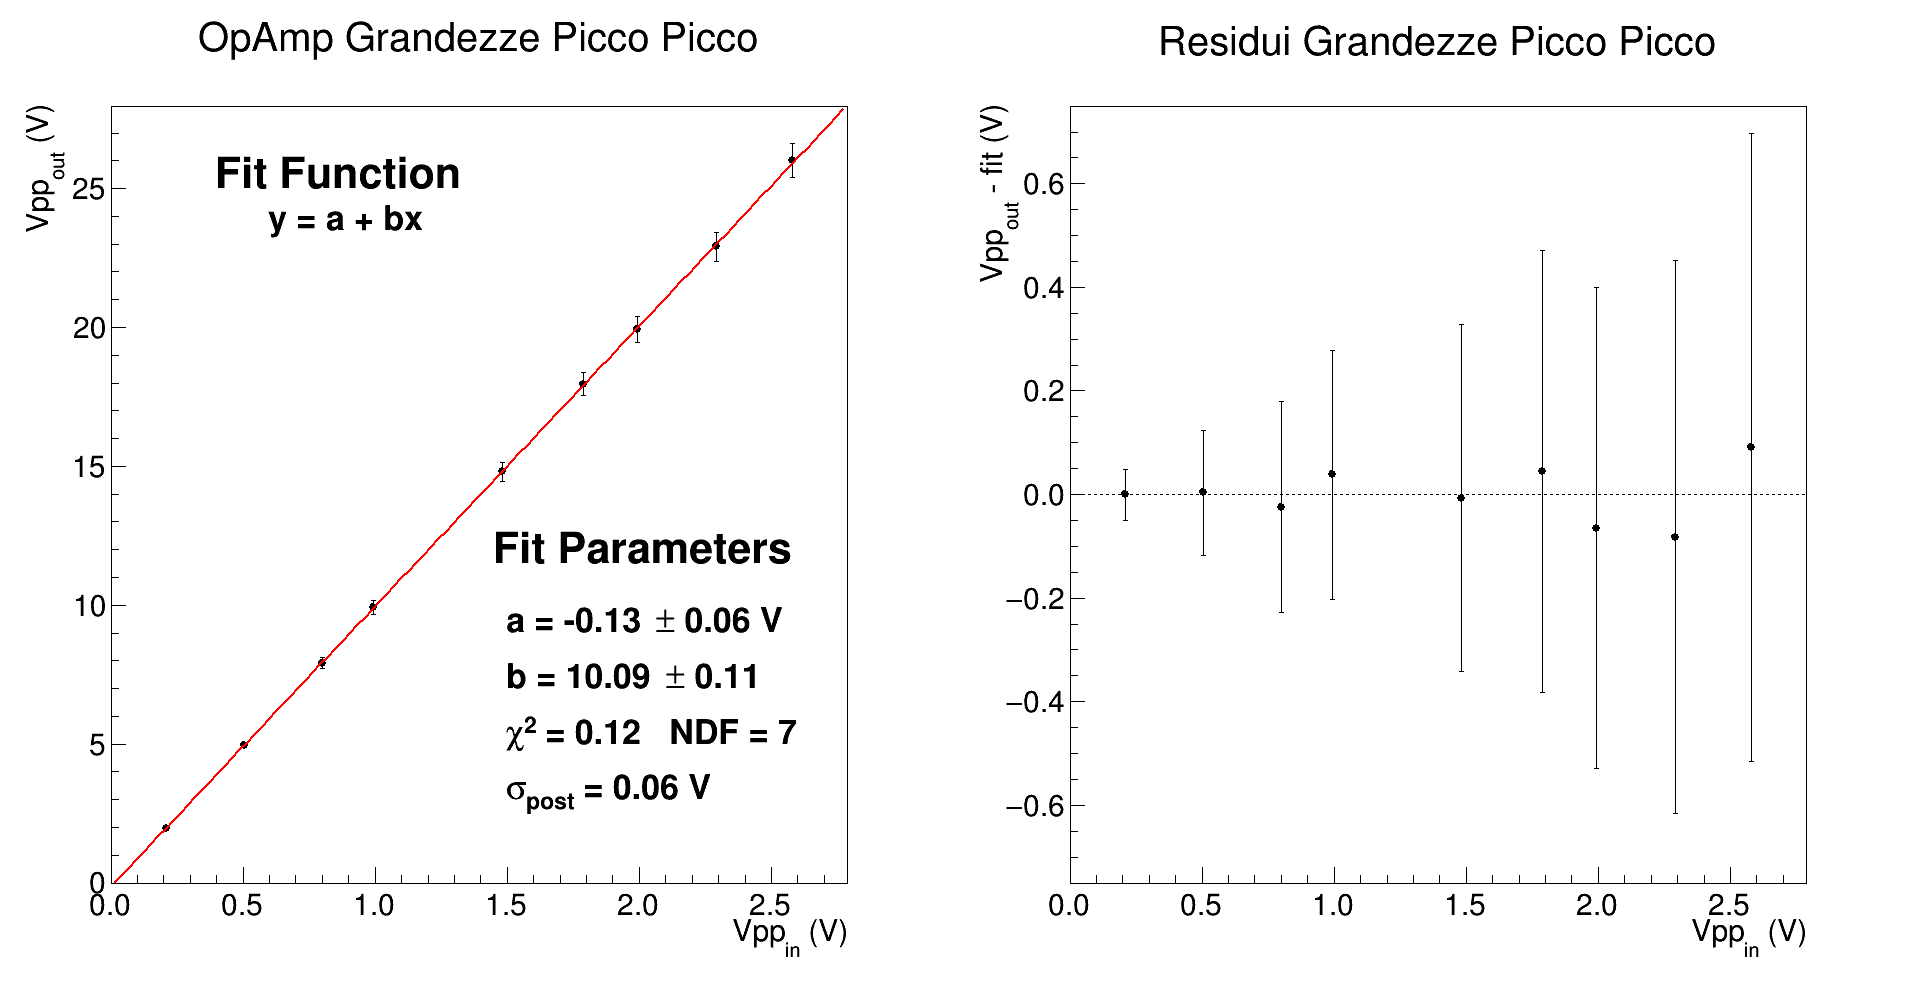
\includegraphics[width=15cm]{../Plots/Report_Plots/opamp_plot_pp_projected.png}
	\caption{A sinistra: grafico rappresentante il dataset delle grandezze picco picco, 
	con relativa retta interpolante e parametri del fit. A destra: grafico dei residui $V\text{pp}_{\text{out}}-\text{fit}$.}
	\label{i:opamp_pp}
\end{figure}

\begin{table}[H]
	\small
	\centering
	\begin{tabular}{x{3cm} x{3cm} x{3cm} x{3cm}} 

		\toprule[0.5px]
		\toprule[0.1px]
		
		\multicolumn{4}{c}{Fit Parameters}\tn
		\midrule[0.1px]

		\addlinespace
		
		Offset (V) & Slope & $\chi^2$/ndf & $\sigma_{\text{posteriori}}$ (V)\tn

		\addlinespace

		$-0.13\pm0.06$ & $10.09\pm0.11$ & $0.12/7$ & $0.06$ \tn

		\bottomrule[0.5px]
		
	\end{tabular}
	\caption{In tabella sono riportati i parametri della retta interpolante, il valore del $\chi^2$ associato al fit 
	e l'errore a posteriori relativo alla distribuzionedelle grandezze picco picco.}
	\label{t:opamp_fitres_pp}
\end{table}	

\noindent Si nota immediatamente, osservando il grafico dei residui, come ora l'andamento anomalo è del tutto assente ed
i punti si distribuiscono in modo ottimale attorno allo zero. Rimane, chiaramente, il tipico andamento crescente delle
barre d'errore, indice che le incertezze continuano a risentire della correlazione tra esse. Il valore del $\chi^2$ è
decisamente basso rispetto al numero di gradi di libertà, come suggerito dal grafico dei residui in cui si nota
chiaramente come la distanza punto-retta sia ampiamente compresa entro la barra d'errore del dato. L'errore a posteriori
è appena maggiore dell'incertezza associata al primo punto, mentre diventa notevolmente inferiore rispetto ai punti
finali. Il valore dell'intercetta, scarsamente compatibile con lo zero, suggerisce una conferma all'ipotesi un una
sistematica di offset/shift verticale tra i due dataset non trascurabile. Il coefficiente angolare, invece, è
perfettamente in linea con i parametri ottenuti considerando i due dataset separatamente: calcolando la media pesata dei
due, infatti, si trova $\langle m\rangle_{\text{max, min}}=10.09 \pm 0.10$ e risulta avere una compatibilità
estremamente elevata con il coefficiente angolare riguardante il dataset delle grandezze picco picco ($\lambda = 0.01$).
Si assume dunque che questi due valori (media pesata dei coefficienti angolari $\langle m\rangle_{\text{max, min}}$ e
coefficiente angolare del campione di grandezze picco picco $m_{\text{pp}}$) rappresentino una soddisfacente stima
dell'amplificazione \textit{G} del circuito. Per quanto riguarda la linearità dell'amplificatore operazionale, invece, i
valori estremamente ridotti del $\chi^2$ non permettono nè di confermare l'ipotesi di linearità nè di poterla rigettare.
Si ripone allora maggior attenzione alla distribuzione delle misure attorno alla retta (o meglio alla distribuzione dei
residui attorno allo zero) che si ritiene invece, in questa occasione, determinante: il campione di misure picco picco
( \autoref{i:opamp_pp}) suggerisce una soddisfacente distribuzione lineare dei dati. 

\subsubsection{Confronto tra Stime di G}
Si vuole ora esporre e confrontare le stime dell'amplificazione del circuito, rappresentando i valori del guadagno
\textit{G} in \autoref{i:opamp_comp}.

\begin{figure}[H]
	\centering
	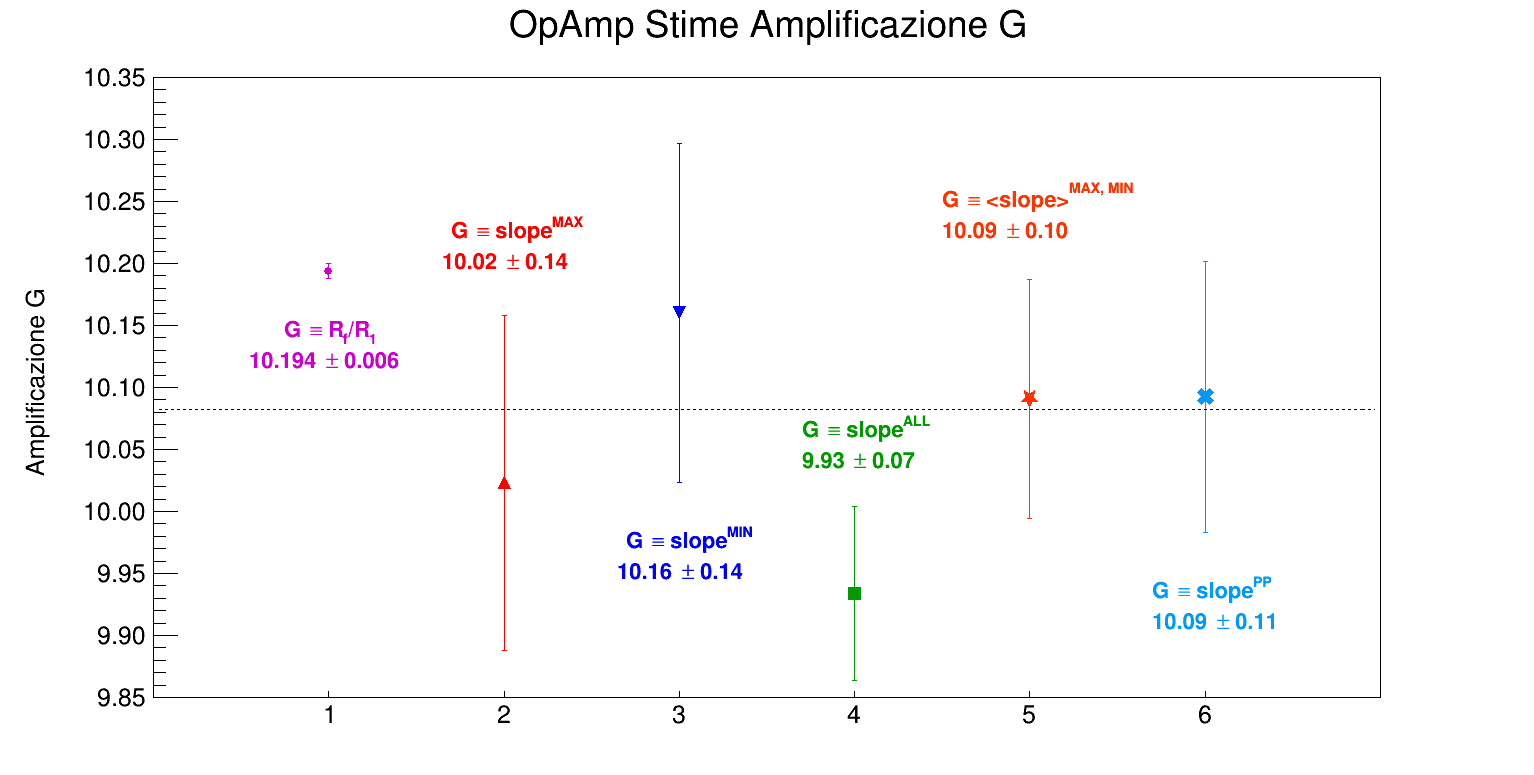
\includegraphics[width=15cm]{../Plots/Report_Plots/opamp_comp.png}
	\caption{Da sinistra: 1) stima di \textit{G} partendo dalle misure dirette delle resistenze del circuito;
	2) stima di G come coefficiente angolare del dataset di massimi; 3) stima di G come coefficiente 
	angolare del dataset di minimi; 4) stima di G come coefficiente angolare del dataset unificato; 
	5) stima di G come media pesata di 2 e 3; 6) stima di G come coefficiente angolare del dataset delle 
	grandezze picco picco.}
	\label{i:opamp_comp}
\end{figure}

\noindent Partendo dal primo punto a sinistra, cioè la stima di \textit{G} tramite le misure dirette delle resistenze
$R_{\text{f}}$ e $R_{1}$ (riportate in \autoref{t:direct_measures}), si nota come questo presenti un errore nettamente
inferiore a confronto con le rimanenti stime. Quest'ultime risultano essere quantità compatibili con 1)
$G=R_{\text{f}}/R_{1}$, ad eccezione di 4) quella ottenuta considerando assieme sia i massimi sia i minimi ($\lambda =
3.7$). In particolare, si può osservare come la media pesata 5) tra le stime dell'amplificazione ottenute considerando i
campioni separati e la stima ottenuta con le grandezze picco picco 6) si trovino in eccellente accordo: si può concludere
dunque che, eliminando la sistematica di offset/shift verticale tra i due dataset (sia attraverso grandezze picco picco,
sia considerando la media pesata dei risultati ottenuti dai campioni separati), la stima dell'amplificazione del
circuito risulta essere compatibile con le aspettative preliminari. Si assume in ogni caso che l'errore su \textit{G}
sia sottostimato a causa della correlazione tra errori di scala dell'oscilloscopio: si preferisce dunque la stima
ritrovata considerando le tensioni picco picco 6), in quanto presenta un errore relativo leggermente maggiore.





\end{document}